\documentclass[12pt,a4paper]{article}
\usepackage[utf8]{inputenc}
\usepackage{amsmath}
\usepackage[brazilian]{babel} % Brazil or not Brazil??
\usepackage{amsfonts}
\usepackage{amssymb}
\usepackage{graphicx}
\usepackage[margin=0.8in]{geometry}


\begin{document}
\title{\vspace{70mm}\Huge Experimento 05 - Viscosidade - Lei de Stokes}
\author{ Giovani Garuffi\qquad\hfill
		\textit {RA: 155559}\protect\\
		João Baraldi\hfill
		\textit{RA: 158044}\protect\\
		Lauro Cruz\hfill
		\textit{RA: 156175}\protect\\
		Lucas Schanner\hfill
		\textit{RA: 156412}\protect\\
		Pedro Stringhini\hfill
		\textit {RA: 156983}								
		}
\maketitle
\newpage
\section{Resumo}


\section{Objetivos}



\section{Procedimento Experimental e Coleta de Dados}


\subsection{Procedimento}

\subsection{Dados Obtidos}

A Tabela \ref{dados} apresenta as medições do tempo de queda de cada esfera, relacionada ao seu raio.

\begin{table}[!htbp]

\centering
\def\arraystretch{1.5}
\caption{Dados obtidos no experimento}

\begin{tabular}{|c|rrrrr|r|}
\hline
$ r \; (m)$ & \multicolumn{5}{c|}{Medidas de $T$ \;  (s)} & $T_{medio} \; (s)$  \\
\hline
  $ 0.00100 \pm 0.00005 $ &12.47 & 12.22 & 11.87 & 11.97 & 11.94 & $ 12.0 \pm 0.3 $ \\
  \hline
  $ 0.00125 \pm 0.00005 $ &7.65 & 7.87 & 7.59 & 7.60 & 7.78  & $ 7.7 \pm 0.3 $   \\
  \hline
  $ 0.00150 \pm 0.00005 $ &5.46 & 5.29 & 5.35 & 5.69 & 5.32 & $ 5.4 \pm 0.3 $     \\
  \hline
  $ 0.00175 \pm 0.00005 $ &4.07 & 4.15 & 4.09 & 4.09 & 4.13  & $ 4.1 \pm 0.3 $    \\
  \hline
  $ 0.00200 \pm 0.00005 $ &3.12 & 3.25 & 3.28 & 3.28 & 3.25 & $ 3.2 \pm 0.3 $       \\
\hline
\end{tabular}

\emph{O erro instrumental em $T$ é considerado $0.3$ devido às dificuldades em realizar as medições}
\label{dados}
\end{table}




\section{Análise dos Resultados e Discussões}
\subsection{Regressão linear}
O situação estudada pode ser modelada a partir da equação: 

$$ v_l = \frac{2}{9} \frac{(\rho - \rho ')}{\eta}g \cdot r^2$$

Obtida a partir da força de empuxo, força gravitacional e da Lei de Stokes. $\rho$ e $\rho '$ são as densidades da esfera e do meio, respectivamente e $\eta$ é o coeficiente de viscosidade do meio.

No entanto a velocidade precisa ser corrigida pelo fator de Landenburg
$$ v_l = K \cdot v_l ' = K \frac{L}{T}$$
$$ \Delta v_l = \sqrt{\frac{K^{2} L^{2}}{t^{4}} \Delta{t}^{2} + \frac{K^{2} \Delta{L}^{2}}{t^{2}} + \frac{L^{2} \Delta{K}^{2}}{t^{2}}} $$
Onde K é o fator de Landenburg, dado por 
$$ K = \left(1 + \frac{3.3 r}{H}\right) \left(1 + \frac{2.4 r}{ \pi r_{c}^{2}}  \right) $$
$$ \Delta K = $$
$$\sqrt{\frac{23.04 \Delta{r_{c}}^{2} r^{2}}{\pi^{2} r_{c}^{6}} \left(1 + \frac{3.3 r}{H}\right)^{2} + \Delta{r}^{2} \left(\frac{2.4 + \frac{7.92 r}{H}}{\pi r_{c}^{2}} + \frac{1}{H} \left(\frac{7.92 r}{\pi r_{c}^{2}} + 3.3\right)\right)^{2} + \frac{10.89 \Delta{H}^{2}}{H^{4}} r^{2} \left(\frac{2.4 r}{\pi r_{c}^{2}} + 1\right)^{2}} $$




Na equaçao  vemos que existe uma relação linear entre $v_l$ e $r^2$. Para explorar essa relação, foi construída a Tabela \ref{linear}, relacionando $v_l$ a $ r^2 $ .

\begin{table}[!htbp]
\centering
\def\arraystretch{1.5}
\caption{O quadrado do raio relacionado à velocidade máxima de uma esfera em um liquido viscoso}
\begin{tabular}{|c|c|c|c|c|}
\hline
$r \; (m)$ & $r^2 \; (m^2)$ & $T_{queda} \; (s)$ & $ K $ & $ v_l \; (m/s)$  \\

\hline
$ 0.00100 \pm 0.00005 $ & $1.0 \cdot 10^{-6} \pm 1 \cdot 10^{-7}$   &$ 12.0 \pm 0.3$ & $ 1.85 \pm 0.04$ & $0.030 \pm 0.001 $\\
 \hline
$ 0.00125 \pm 0.00005 $ & $1.5 \cdot 10^{-6} \pm 1 \cdot 10^{-7}$ & $ 7.7 \pm 0.3$ & $ 2.07 \pm 0.04$  & $0.053 \pm 0.002 $\\
 \hline
$ 0.00150 \pm 0.00005 $ & $2.2 \cdot 10^{-6} \pm 2 \cdot 10^{-7}$ & $ 5.4 \pm 0.3$ & $ 2.28 \pm 0.04$  & $0.084 \pm 0.005 $\\
 \hline
$ 0.00175 \pm 0.00005 $ & $3.0 \cdot 10^{-6} \pm 2 \cdot 10^{-7}$ & $ 4.1 \pm 0.3$ & $ 2.50 \pm 0.04$   & $0.121 \pm 0.009 $ \\
 \hline
 $0.00200 \pm 0.00005 $ & $4.0 \cdot 10^{-6} \pm 2 \cdot 10^{-7}$   & $ 3.2 \pm 0.3$ & $ 2.71 \pm 0.04$   & $0.16 \pm 0.01 $\\
\hline
\end{tabular}

\emph{O erro em T foi calculado pelo erro estatístico e utilizando como  erro instrumental $\pm 0.3$}
 
\label{linear}
\end{table}

Fazendo a regressão linear de $ v_l$ X $ r^2 $, pelo método de mínimos quadrados, obtém-se os seguintes coeficientes: 
	$$ a = (41 \pm 2) \cdot 10^3  \;\; (1/ms)$$
	$$ b = 0.011 \pm 0.003 \; (m/s).$$

A reta resultante da regressão linear, sobreposta aos pontos medidos experimentalmente pode ser vista na Figura \ref{grafico}.

\begin{figure}
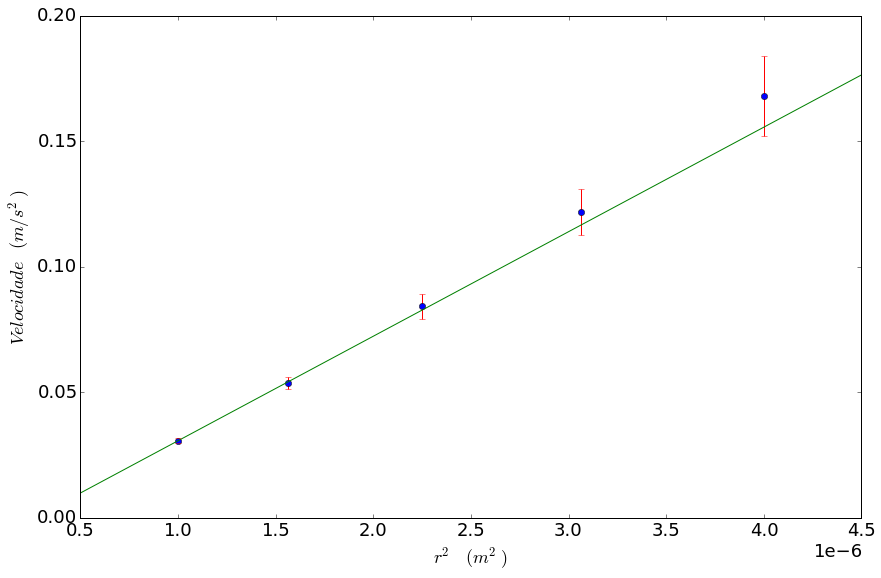
\includegraphics[scale=0.55]{grafico.png}
\caption{Regressão linear de $v_t$ por $r^2$ sobreposta aos pontos experimentais}
\label{grafico}
\end{figure}

\subsection{Significado físico do coeficiente angular}



\section{Conclusões}

\end{document}

